\documentclass{whutmod}
\usepackage[linesnumbered,ruled,lined]{algorithm2e}
\usepackage{diagbox}
\bibliographystyle{unsrt}
\team{10}
\membera{刘子川}
\joba{编程}
\memberb{程宇}
\jobb{建模}
\memberc{祁成}
\jobc{写作}
\hypersetup{
	colorlinks=true,
	linkcolor=black,citecolor=black
}


\newcommand{\upcite}[1]{\textsuperscript{\cite{#1}}}
%%%%%%%%%%%%%%%%%%%%%%%%%%%%%%%%%题目%%%%%%%%%%%%%%%%%%%%%%%%%%%%%%%%%%%%
\title{基于NSGA-II算法的插板式编码\\多目标优化生产调度模型}
\tihao{5} 
\everymath{\displaystyle}
\begin{document}

	\maketitle
	\thispagestyle{empty}
%%%%%%%%%%%%%%%%%%%%%%%%%%%%%%%%%摘要%%%%%%%%%%%%%%%%%%%%%%%%%%%%%%%%%%%%
	\begin{abstract}
		
		控制高压油管的压力变化对减小燃油量偏差,提高生产计划效率具有重要意义。本文建立了兼顾全局一体化的多目标优化调度模型,采用插板编码的\textbf{NSGA-II算法}对模型进行求解,并从帕累托前沿解中求得最短工艺生产时间。

		\vspace{7pt}	%空格

		针对炼钢、连铸、热轧工艺过程特点,列举模型的约束条件。对于转炉、连铸机与热轧机而言其各炉次、浇次、轧制单元的生产量\textbf{存在上下限}。在炼钢过程中每炉次只可使用同种钢材,在连铸过程中每浇次最多可\textbf{生产两种型号}的钢坯。对每个轧制单元而言,需存在一定比例的热棍材与主体材,且在轧制顺序上的相邻钢坯硬度、宽度和厚度需保证\textbf{单调增长}且不能大幅度变化。

		\vspace{8pt}	%空格

		针对问题二,基于问题一整理归纳特点,建立炼钢、连铸、热轧一体化生产多目标优化模型。首先为使得转炉、连铸机和热轧机的闲置产能最低,本节将其各炉次、浇次、轧制单元的空闲产能分别求和并作为\textbf{多目标优化}中的目标函数。之后分别根据各炼钢、连铸、热轧的工艺特点,列举每个生产过程中的约束条件。在设计\textbf{插板式编码}作为编码方式后,采用\textbf{NSGA-II}算法求解该多目标优化的\textbf{帕累托前沿},并在帕累托前沿中选择生产时间最低的解作为最终生产方案。

		针对一体化调度问题,基于其归纳的特点及约束,建立炼钢、连铸、热轧一体化生产多目标优化模型。首先为使得转炉、连铸机和热轧机的闲置产能最低,本节将其各炉次、浇次、轧制单元的空闲产能分别求和并作为\textbf{多目标优化}中的目标函数。之后分别根据各炼钢、连铸、热轧的工艺特点,列举每个生产过程中的约束条件。在设计\textbf{插板式编码}作为编码方式后,采用\textbf{NSGA-II算法}求解该多目标优化的\textbf{帕累托前沿},并在帕累托前沿中选择生产时间最低的解作为最终生产方案。
		\vspace{8pt}	%空格
		
		文中以某钢铁联合企业为研究对象进行仿真测试。仿真过程中NSGA-Ⅱ算法在CPU Intel T5800 1.6GHz, 2GB内存环境下进行多次实验。结果表明设置轧制单元个数为13个时,经快速非支配排叙最终得到\textbf{非支配解有11个}最优解,求得在满足约束条件下完成前十个订单的\textbf{最短时间为36580min}。最后本文调整插板个数并做出灵敏度分析,分析结果表示NSGA-II算法具有\textbf{较强稳定性}。
		\vspace{8pt}	%空格			

		本文的优点为:1. 本文多维度考虑生产效率对全局的依赖,并在符合严苛的工艺约束条件下全局求得单元计划排列顺序,利用帕累托前沿解大幅缩短工艺生产时间。2.针对智能算法求解方面,使用NSGA-II算法并巧妙采用插板式编码方式对多目标优化求解,兼顾局部搜索与全局搜索能力。
		
		
		\keywords{
			NSGA-II算法\quad
			插板式编码\quad	
			帕累托前沿解\quad
			多目标优化调度模型\quad
		}
	\end{abstract}


%%%%%%%%%%%%%%%%%%%%%%%%%%%%%%%%%目录%%%%%%%%%%%%%%%%%%%%%%%%%%%%%%%%%%%%
	\thispagestyle{empty}
	\tableofcontents
	\setcounter{page}{0}                                      
	\newpage	%换页符
	

	
	\section{问题重述}	
		\subsection{问题背景}
	    随着我国经济发展进入新常态,钢铁行业发展环境发生了深刻变化。2015年,我国钢铁消费与产量双双进入峰值弧顶区并呈下降态势,钢铁主业从微利经营进入整体亏损,行业发展进入“严冬”期。钢铁行业要落实中央经济工作会议精神,着力推进供给侧结构性改革,扎实完成《国务院关于钢铁行业化解过剩产能实现脱困发展的意见》的各项部署和要求。在化解产能过剩的同时,也将注重产业结构优化和升级,做好规范企业动态管理、智能制造试点示范、钢结构建筑推广应用等重点工作,引领钢铁工业提高综合竞争力。
	    
	    炼钢、连铸和热轧作为钢铁生产的关键工序,工序之间不仅仅是物流与信息流的交换,还存在能量平衡和时间平衡。炼钢一连铸一热轧一体化生产计划编制是通过多个模块、多个模型互相协作来完成,整个生产计划编制过程按照一定的时间长度周期性进行。在每一个计划编制周期内, 具体编制流程如图~\ref{111111}~所示。面向订单组织生产管理思想以及炼钢、连铸和热轧一体化排程使各工序的物流控制以及计划之间具有很好的继承性,可以最大限度地减少物料在工序间的停留时间,缩短制造周期和交货周期,还可以减少温降和能量损失、节约能源、降低生产成本。
				\begin{figure}[H]
		\centering
		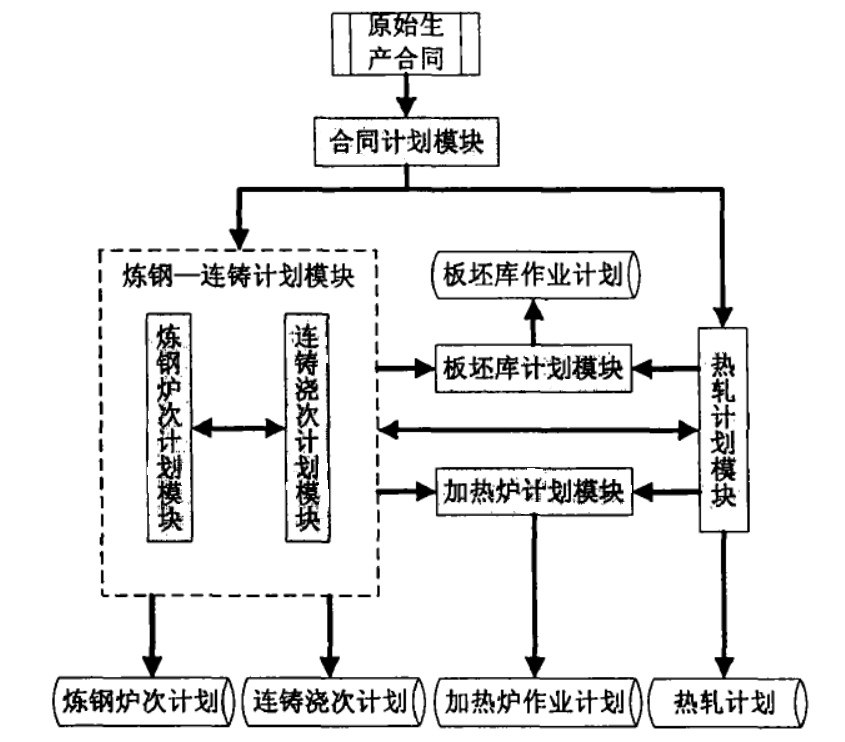
\includegraphics[width=.8\textwidth]{figures/asd.png}
		\caption{一体化计划编制流程}\label{111111}
	\end{figure}
		\subsection{问题概述}
		    围绕某钢厂生产数据附件和条件要求,研究炼钢、连铸和热轧一体化生产的调度方案,依次提出以下问题:
				 
			
			\textbf{特点:}说明炼钢、连铸、热轧一体化生产组织、工艺过程特点。
			
			\textbf{模型:}建立炼钢、连铸、热轧一体化生产计划数学模型。
			
			\textbf{仿真:}利用附件 1 中某钢厂的实际生产数据,仿真验证前面所建模型。

	
	\section{模型假设}

\begin{itemize}                                             
	\item [(1)] 假设各工序间的成品的物流时间非常短暂,可以忽略不考虑。
	\item [(2)] 假设每次连铸、热轧的准备时间相同,不会随着工作次数变化而发生变化。
	\item [(3)] 假设浇铸、热轧每块刚材的所需时间相同,不会因为钢材的型号类型不同而发生变化。
	\item [(4)] 不考虑制作过程中能量损失,即忽略炼钢、连铸和热轧过程中的材料温度下降。
\end{itemize}



		
	\section{符号说明}
		\begin{table}[H]
		\centering
		\setstretch{1.2}  %设置表的行间距
		\setlength{\tabcolsep}{12mm}
		\begin{tabular}{cc}
			\toprule[1.5pt]
			\multicolumn{1}{m{4cm}}{\centering 符号} & \multicolumn{1}{m{6cm}}{\centering 说明} \\
			\midrule[1pt]		
			$c_i, l_i, w_i, t_i, h_i$  & 板坯属性  \\ 
				$c'_i, l'_i, w'_i, t'_i, h'_i$  & 卷钢属性  \\ 
		   	$Molten_i, Bar_i, Strip_i$  & 单份钢水、单份板坯、单份卷钢  \\
		   	$Heat_j, Cast_k, Roll_j$  & 单个炉次、浇次、热轧单元计划  \\ 
		 $f_1, f_2, f_3$  & 各计划空闲连铸机容量之和 \\   
		  $[n_{alter}]$  & 变化次数的许用阈值 \\   
		   $[\Delta w]$  & 板坯宽度的许用变化量 \\
		 $t_{Cast}, t_{Roll}$  & 一次浇铸、轧制操作需要的准备时间 \\  
		 $t_{bar}, t_{Strip}$  & 浇铸、轧制一份刚卷需要的时间 \\     
			\bottomrule[1.5pt]
		\end{tabular}
		\begin{tablenotes}
		\item 注:表中未说明的符号以首次出现处为准
		\end{tablenotes}
		\end{table}

	
	\newpage
	\section{炼钢、连铸、热轧一体化生产组织、工艺过程特点}
	 钢铁生产是一个高温、高能耗、物流量巨大的加工过程,整个生产流程工艺复杂,工序很多,各工序的工艺约束和生产调度目标也不尽相同\upcite{1,2}。高效实用的钢铁生产调度必须建 立在对钢铁生产流程的充分了解基础之上,特别是必须充分考虑到近年来钢铁生产技术的两大飞跃:连铸与热送热装轧制对于生产调度技术的影响\upcite{1,3,4}。
	 
	 一个典型的钢铁企业的生产流程如图~\ref{1111ss11}~所示,可分为三大部分:炼铁区域(Iron Making)、主炼钢区域(Primary Steelmaking)和精整加工区域。其中主练钢包括炼钢、连铸、热轧等工序。
	\begin{figure}[H]
		\centering
		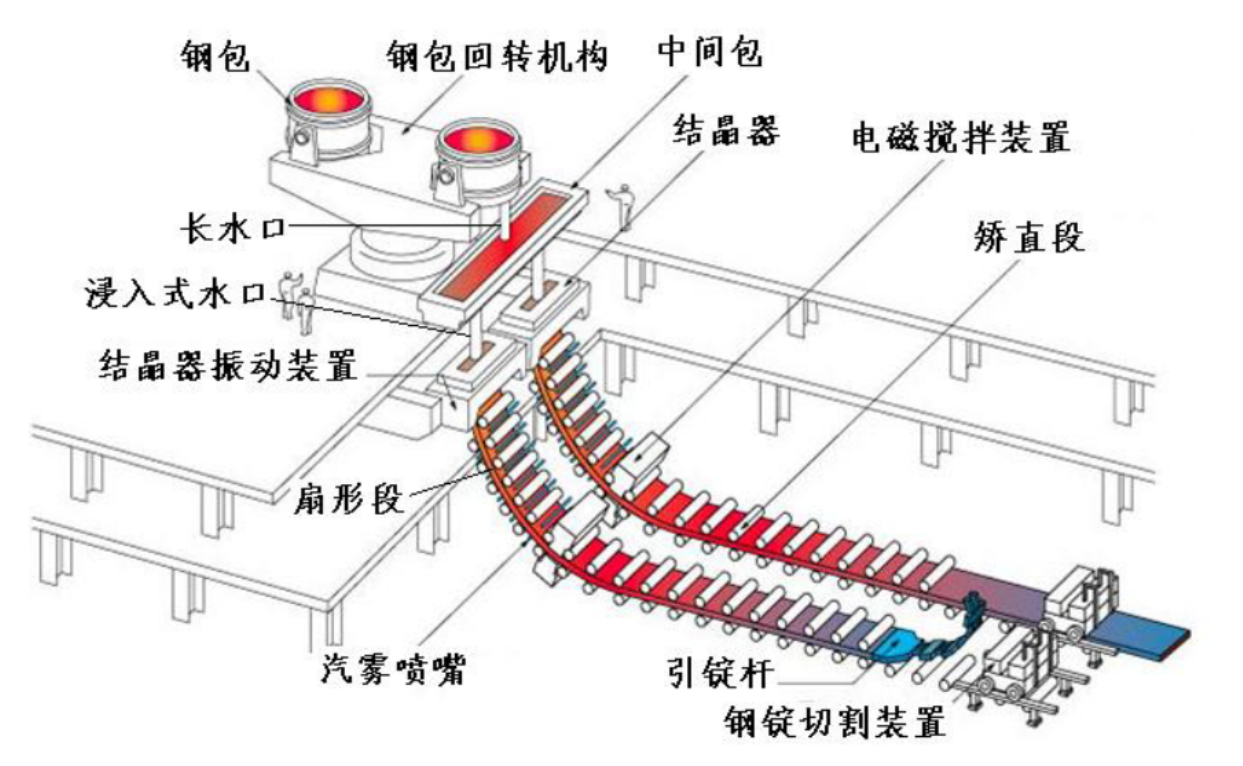
\includegraphics[width=.9\textwidth]{figures/sda.png}
		\caption{钢铁生产工艺示意图}\label{1111ss11}
	\end{figure}

		
\subsection{基本物流要素和流动体系表示}


\textbf{定义}物流传递过程中的主物流等价概念:单份钢水$Molten_i$、单份板坯$Bar_i$、单份卷钢$Strip_i$,三者是不同表现形式的同一物质;同样可定义工序概念:单个炉次$Heat_j$、单个浇次$Cast_k$、单个热轧单元计划$Roll_j$,三者是同一物质的不同量度。
\vspace{7pt}	%空格
		
\textbf{定义}一个单元计划包含的所有板坯的集合为$Bar$,单个板坯记为$Bar_i$,每个板坯具有属性:钢种$c_i$、长度$l_i$、宽度$w_i$、厚度$t_i$、硬度$h_i$。
		\vspace{7pt}	%空格
		
\textbf{定义}单个卷钢为$Strip_i$,每个卷钢由板坯经过物理变化得到,视为板坯的变形体,具有与板坯完全相似属性:钢种$c'_i$、长度$l'_i$、宽度$w'_i$、厚度$t'_i$、硬度$h'_i$。

不考虑加工过程中物质传递损失,则三种主物流与三种工序的关系为
\begin{gather}
\left\{\begin{matrix}
Heat_j=\sum_{i=1}^{n_{Molten}}Molten_i,
\\Cast_k=\sum_{i=1}^{n_{Bar}}Bar_i,
\\ Roll_j=\sum_{i=1}^{n_{Strip}}Strip_i.
\end{matrix}\right.
\end{gather}

其中假设多个炉次对应于一个浇次,一个浇次对应于一个热轧单元计划。则有
$Roll_j=Cast_j=\sum_{u=1}^{n_{heat}}Heat_u=\sum_{u=1}^{n_{heat}}Heat_u=\sum_{j=1}^{n_{Heat}}\sum_{i=1}^{n_{Molten}}Molten_{ij}.$因此因此,总物流表示为
\begin{gather*}
F=\sum_{j=1}^{n_{Roll}}Roll_j=\sum_{j=1}^{n_{Cast}}Cast_j=\sum_{k=1}^{n_{Roll}}\sum_{u=1}^{n_{Heat}}Heat_u=\sum_{h=1}^{n_{Roll}}\sum_{j=1}^{n_{Heat}}\sum_{i=1}^{n_{Molten}}Molten_{ijh}.
\end{gather*}

	\subsection{炼钢、连铸生产动态调度特点}

钢铁企业中典型的生产线一般为多座转炉、多台连铸机和一台热轧机顺序生产,如图~\ref{111sad1sssssss11}~所示。由于转炉和连铸机都是批量加工的设备,炼钢一连铸生产调度属于一类带有批量约束的并行多机的调度问题\upcite{2}。

	\begin{figure}[H]
	\centering
	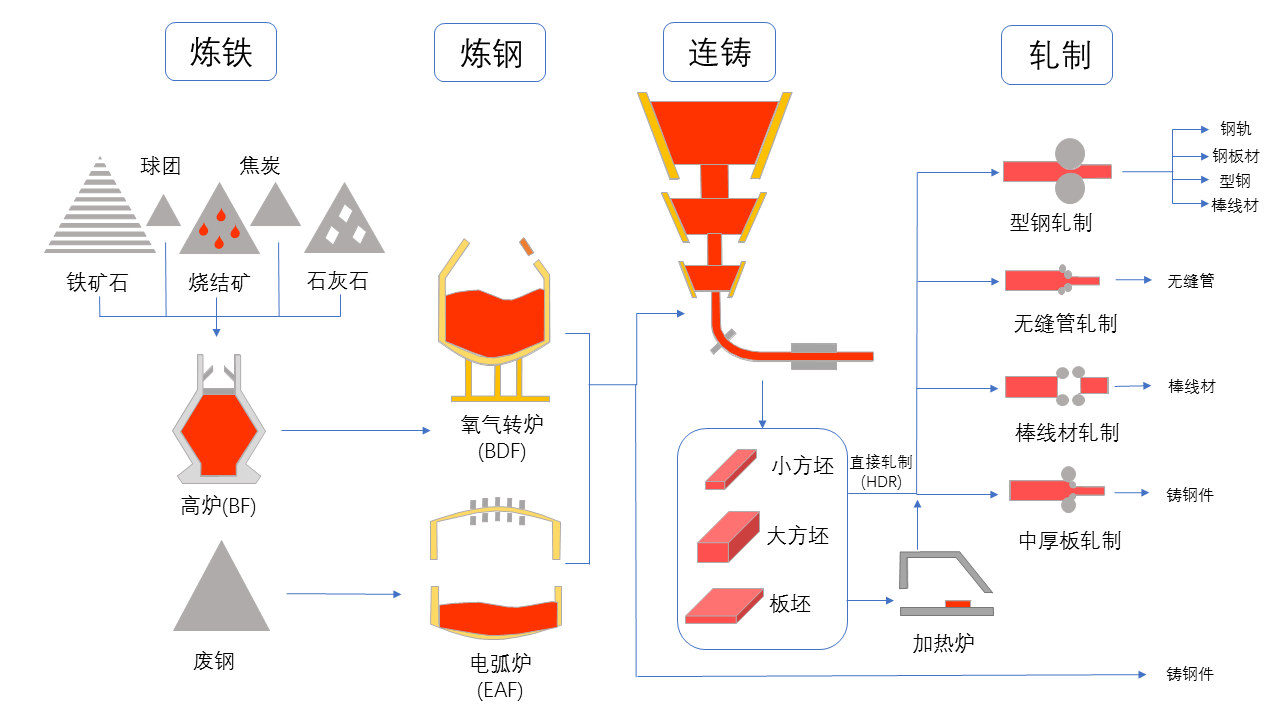
\includegraphics[width=.8\textwidth]{figures/big.png}
	\caption{炼钢、连铸生产流程示意图}\label{111sad1sssssss11}
\end{figure}

    文\upcite{3}中提到由于高炉持续不断地向下游工序提供铁水,所以在炼钢一连铸生产中不会出现工件随机到达或到达时间不确定的情况。炼钢一连铸生产动态调度要求根据出现的动态事件,对原有的生产计划进行调整,使得在满足工艺约束的前提下调整后的调度方案在某一指标上达到最优\upcite{3}。

本文研究的加工时间可控的炼钢-连铸调度问题具有以下\textbf{约束条件}:\\
(1)同一生产设备在同一时段只能加工一个炉次;\\
(2)相邻炉次之间,后一炉次必须等待前一炉次加工完成后才能开始加工;\\
(3)相邻浇次之间,后一阶段的加工开始时刻晚于前一阶段加工完成和设备间运输完成;\\
(4)同一炉次内,后一阶段的加工开始时刻晚于前一阶段加工完成和设备间运输完成;\\
(5)存在不同程度的扰动,各个炉次在不同生产阶段的加工时间可以在一定范围内调整。

	\subsection{热轧生产计划编制问题特点}
%板坯厚度通常为$120-300mm$,最厚达$350mm$,宽度一般与轧成的钢带宽度相同或大于钢带宽度$50-100mm$;热轧带钢是成卷的钢板,厚度介于$0.8-25mm$之间,宽度在$2500-900mm$之间。
如图~\ref{1111sssss11}~所示,精轧机组一般由6—7个机架组成连轧,在精轧加工过程中要用到两类轧辊:工作辊和支撑辊,其中工作辊直接和板坯接触,支撑辊对工作辊起到支撑作用\upcite{5}。每一个机架上的工作辊和支撑辊由于高温高速轧制,轧辊磨损很大。轧辊磨损到一定程度,\textbf{每轧制一定数量的板坯后需要更换轧辊}。为了降低生产成本每个轧制单元轧制的带钢总长度在小于给定的可以轧制的最大带钢轧制长度的前提下要尽可能大\upcite{5}。
	\begin{figure}[H]
	\centering
	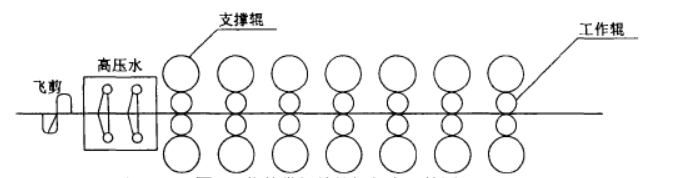
\includegraphics[width=1.05\textwidth]{figures/demo.png}
	\caption{热轧带钢精轧机组布置简图}\label{1111sssss11}
\end{figure}
 每个轧制单元由两部分组成:烫辊材和主体材在轧制单元的初始阶段为了使轧辊型达到热平衡和稳定,安排轧制烫辊材。烫辊材在轧制单元中所占比例很小,一般安排硬度较低的带钢。紧跟在烫辊材之后的是主体材,生产合同绝大多数都是在主体材阶段轧制完成。


	
	在编制热轧批量计划时必须遵守如下\textbf{工艺约束}:
                                          
	\textbf{对于批量计划:}烫辊材的宽度递增变化,主体材的宽度递减变化。如图~\ref{11sssss11}~所示,一个完整的的轧制单元的带钢宽度具有“双梯形结构”\upcite{6}。
	
	    \textbf{对于烫辊材部分:}烫辊材长度有一定限制;烫辊材宽度渐增变化,变化范围有限制轧制的带钢硬度不能太大;硬度变化幅度要小,变化尽量平滑;厚度变化幅度要小,最好是非减方向变化。
	
	\textbf{ 对于主体材部分:}主体材总长度有一定限制;主体材宽度非增方向变化,跳跃幅度要小;宽度、厚度、硬度不允许同时跳跃;厚度变化要平稳,不能反复跳跃,同时最好是非减方向变化;硬度变化要平稳,渐近递增或渐近递减均可,只是不能反复跳跃;当三者发生冲突时,优先级为硬度→厚度→宽度。
	\begin{figure}[H]
		\centering
		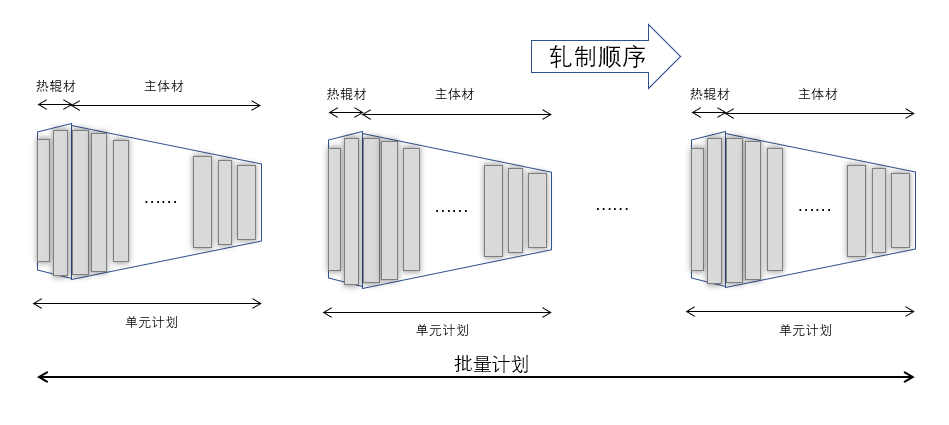
\includegraphics[width=1\textwidth]{figures/asdad.png}
		\caption{热轧批量计划示意图}\label{11sssss11}
	\end{figure}
    

    根据上述分析,热轧批量计划编制的目标选取应满足:在保证产品交货期的前提下,保证产品硬度方面的跳跃最小;保证产品厚度方面的跳跃最小;保证产品宽度方面的跳跃最小。

	
	
	
	\section{一体化调度问题模型的建立与求解}
		\subsection{问题描述与分析}
			问题二要求建立炼钢、连铸、热轧一体化生产计划数学模型。整理文献资料可知\upcite{1,2,3},炼钢、连铸、热轧的工艺特点,一体化调度的主要目标在于优化各设备使用率的同时尽可能降低生产时间,即该一体化调度模型为多目标组合优化模型。
			
			从提高各设备使用率的角度出发,我们将规划各炉次、浇次及轧制单元的生产清单以最大限度的降低设备的闲置产能。由于炼钢、连铸与热轧工艺为顺承关系,本文优先每个规划轧制单元的生产计划,再由此计划逆推各浇次及各炉次的生产清单。其中各轧制单元需存在一定比例的热棍材与主体材,且相邻的轧制板之间的硬度、宽度与厚度的变化不能跳跃式变化。且每个浇次最多可生产两种类型的板材,每个炉次只能生产同种类型的钢水。
			

            当各设备使用率达到最优时,我们认为生产中的非必要能量损耗将降至最低。本文以各设备的闲置产能为多目标优化中的目标函数,通过$NSGA-II$算法求解其对应的帕累托前沿,并在帕累托前沿中选取总生产时间最小的解作为最终方案。

		\subsection{生产优化目标}
		\subsubsection{产能目标函数}
		为降低生产成本,我们将尽可能降低每次生产时的闲置产能。炼钢阶段将优化组炉的空闲炉容量,对每炉次钢水,尽可能降低该炉次的空闲炉容量,即
		\begin{gather}
	    min	f_1=\sum_{v=1}^{n_{heat}}( V_1-\sum_{u=1}^{n_{Molten}} Molten_u),
		\end{gather}
		其中$V_1$表示转炉最大容量,$n_{Heat}$表示总炉次,$n_{Molten}$表示炉次$v$加工的钢水份数,$Molten_u$表示炉次$v$加工的单份钢水的重量。即$f_1$表示每炉次的空闲炉容量之和。同理在连铸阶段时,有
		\begin{gather}
		min	f_2=\sum_{v=1}^{n_{cast}}( V_2-\sum_{u=1}^{n_{Bar}} Bar_u),
		\end{gather}
		其中$V_2$表示连铸机最大容量,$n_{cast}$表示总浇次,$n_{Bar}$表示浇次$v$加工的钢坯份数,$Bar_u$表示浇次$v$加工的第$u$份钢坯的重量。即$f_2$表示每浇次的空闲连铸机容量之和。同理在热轧阶段时,有
		\begin{gather}
		min	f_3=\sum_{v=1}^{n_{Roll}}( V_3-\sum_{u=1}^{n_{Strip}} Strip_u),
		\end{gather}
		其中$V_3$表示热轧机最大轧制长度,$n_{Roll}$表示总轧制单元数,$n_{Strip}$表示浇次$v$加工的钢卷份数,$Strip_u$表示轧制单元$v$加工的第$u$份钢卷的厚度。即$f_3$表示每个轧制单元的空闲轧制长度之和。空闲产能优化实意图如图~\ref{xdffdx}~所示
		\begin{figure}[H]
			\centering
			\subfigure{
\includegraphics[height=3cm,width=5cm]{figures/f1.png}}
			\subfigure{
\includegraphics[height=4cm,width=5cm]{figures/f2.png}}
			\subfigure{
\includegraphics[height=4cm,width=5cm]{figures/f3.png}}
			\caption{空闲产能示意图}\label{xdffdx}
		\end{figure}
		即产能优化目标可表示为
			\begin{gather}
		min \left\{\begin{matrix}f_1=\sum_{v=1}^{n_{heat}}( V_1-\sum_{u=1}^{n_{Molten}} Molten_u),
			\\ f_2=\sum_{v=1}^{n_{cast}}( V_2-\sum_{u=1}^{n_{Bar}} Bar_u),
			\\ f_3=\sum_{v=1}^{n_{Roll}}( V_3-\sum_{u=1}^{n_{Strip}} Strip_u).
		\end{matrix}\right.
			\end{gather}
	   
		\subsubsection{时间目标函数}
		为最大限度的减少物料在工序间的停留时间,本文将在产能目标函数达到最优的情况下尽使得热轧时间与浇铸时间达到之和为最小值。由附件$1$可知,共有两台连铸机,即连铸机工作总时间$T_{cast}$可表示为
		\begin{gather*}
		T_{Cast}=\frac{1}{2}\sum_{i=1}^{n_{Cast}}(n_{Bar}\times t_{Bar}+t_{Cast}),
		\end{gather*}
		其中$t_{Cast}$表示一次浇铸操作需要的准备时间,$t_{bar}$表示浇铸每块钢坯需要的时间。同理热轧机的工作总时间$T_{roll}$可表示为
		\begin{gather*}
		T_{Roll}=\sum_{i=1}^{n_{Roll}}(n_{Strip}\times t_{Strip}+t_{Roll}),
		\end{gather*}
		其中$t_{Roll}$表示一次轧制需要的准备时间,$t_{Strip}$表示轧制一份刚卷需要的时间。由于转炉总数未知,且一般炼钢厂转炉数量较多,我们将不把炼钢总时间归入时间目标函数,即时间目标函数$T$可表示为
	    \begin{gather}
		minT=T_{Cast}+T_{Roll}.
		\end{gather}
		本文将优先计算使得产能目标函数最优时的帕累托解平面,然后在解平面中选择时间目标函数最优解作为最终生产方案。
		
			
		\subsection{工艺约束条件}
		根据工序划分,有组炉约束、组浇约束和热轧单元约束三大约束条件,并存在时间网络约束如下图所示
			\begin{figure}[H]
			\centering
			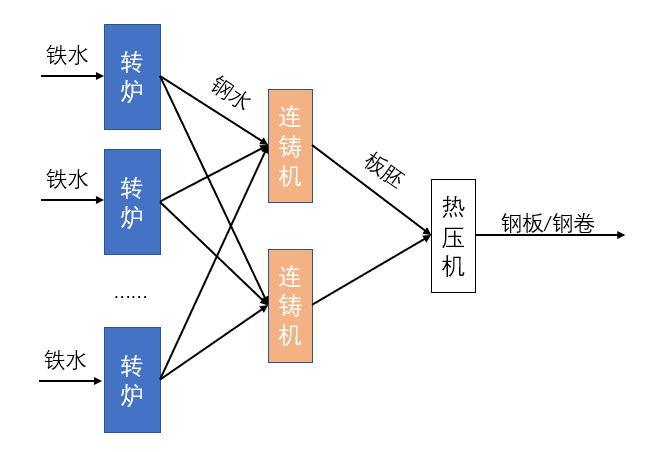
\includegraphics[height=6cm,width=.7\textwidth]{figures/faf.png}
			\caption{工序时间约束网络}\label{111sad1sssasdssss11}
		\end{figure}
		
		
		\subsubsection{组炉约束}
		各个工序的生产工艺约束对于炼钢工序的炉次计划,组成同一炉次的合同必须满足:(1)钢级相同;(2)板坯宽度相同;(3)轧制宽度≤板坯宽度≤轧制宽度+100mm;(4)厚度相同;(65)95\%炉容量≤板坯总重量≤100\%炉容量。
		
		一个炉次中,
		\textbf{组炉约束}描述如下:
		\begin{gather}
		\left\{\begin{matrix}
		c_i=c_0,
		\\ t_i=t_0,
		\\ w_i=w_0\geq 140,
		\\ w_i'\leq w_i\leq w_i'+100,
		\\ 95\% \cdot \sum_{u=1}^{n_{Heat}}Heat_u\leq\sum_{i=1}^{n_{Bar}}Bar_i\leq\sum_{u=1}^{n_{Heat}}Heat_u.
		\end{matrix}\right.
		\end{gather}
		
		\subsubsection{组浇约束}
		多个炉次构成一个浇次。组成同一浇次的炉次之间必须满足如下条件:(1)钢级的要求,不同炉次之间的钢级存在的关系如表\ref{biao1}所示:
		\begin{table}[H]
			\setstretch{1.0}  %设置表的行间距
			\centering		
			\caption{炉次间的钢级关系}\label{biao1}
			\begin{threeparttable}
			\begin{tabular}{ccccc}
				\toprule[2pt]
				\multicolumn{1}{m{2cm}}{\centering 炉次\tnote{1}}
				& \multicolumn{1}{m{2cm}}{\centering $C_1$}
				& \multicolumn{1}{m{2cm}}{\centering $C_2$}
				& \multicolumn{1}{m{2cm}}{\centering $C_3$}
				& \multicolumn{1}{m{2cm}}{\centering $C_4$}
				\\
				\midrule[1pt]
				$C_1$ &0&1&2&3\\ 
				$C_2$ &1&0&3&2\\ 
				$C_3$ &2&3&0&3\\ 
				$C_4$ &3&2&3&0\\ 
				\bottomrule[2pt]	
			\end{tabular}
		\begin{tablenotes}
			\footnotesize
			\item[1]$C_i$是第$i$个炉次对应的钢级;0-钢级完全相同可直接连浇;1—钢级相近不用隔板,可直接连浇;2—用隔板进行质量分离连浇;3-不能连浇。
		\end{tablenotes}
		\end{threeparttable}
		\end{table}
		(2)炉次之间的板坯厚度一致。根据国家标准《连铸工程设计规范》GB\ 50580-2010,板坯厚度不宜小于$140mm$;(3)板坯的宽度变化不允许超过一定次数;(4)如果不同宽度的炉次组成同一浇次,一般是按宽度非增顺序排列,而且变化不能太大。
		
		对浇次$Cast_k$中的任意板坯$Bar_j$和$\Delta Bar_j$,\textbf{组浇约束}描述如下:
		\begin{gather}
		\left\{\begin{matrix}
		w_{j+1}\leq w_{j},
		\\ |\Delta w_j|\leq [\Delta w],
		\\\sum_{j=1}^{n_{w}-1}[\frac{|\Delta w_j|}{[|\Delta w_j|]}]\leq [n_{alter}],
		\end{matrix}\right.
		\end{gather}
		其中,$[n_{alter}]$是变化次数的许用阈值,$[\Delta w]$是板坯宽度的许用变化量。
		\subsubsection{热轧单元约束}

		工程上对于板坯具有的某一属性(宽度、厚度、硬度),需要满足属性值不超过许用属性值,且在轧制单元计划中,相邻两板坯的属性变化量不得超过许用属性变化量。则对单元计划中第$i$块板坯的属性$x_i$有
		\begin{gather}
		0\leq \Delta x_i=x_i-x_{i+1}\leq [\Delta x].
		\end{gather}
		
		考虑到工作压辊更换成本与属性变化正相关,需要限制板坯属性变化总量
		\begin{gather*}
		\sum_{i}^{n-1}\Delta x_i\leq X_0,
		\end{gather*}
		同时,属性变化不能反向跳跃,即
		\begin{gather*}
		\Delta x_i\cdot \Delta x_{i+1}\geq 0.
		\end{gather*}
		
		最后,板坯的硬度、厚度、宽度三种属性具有递减的优先级,为简化模型,限制相邻板坯之间只有一个属性变化,即
		\begin{gather}
		[\frac{|\Delta w_j|}{[|\Delta w_j|]}]+[\frac{|\Delta t_j|}{[|\Delta t_j|]}]+[\frac{|\Delta h_j|}{[|\Delta h_j|]}]\leq 1.
		\end{gather}
		
		加以板坯总长度限制,可以得到热轧单元总约束为:
		\begin{gather}
		\left\{\begin{matrix}
		\Delta t_j\cdot \Delta t_{j+1}\geq 0,
		\\\Delta h_j\cdot \Delta h_{j+1}\geq 0, 
		\\\textstyle \sum_{j=1}^{n}Roll_{j}\leq B_0,
		\\ \textstyle\sum_{j}^{n-1}\Delta w_i\leq W_0,
		\\\textstyle\sum_{j}^{n-1}\Delta t_i\leq T_0,  
		\\0\leq\Delta t_j=t_{j}-t_{j+1}\leq [\Delta t],
		\\0\leq\Delta w_j=w_{j}-w_{j+1}\leq [\Delta w],
		\\ [\frac{|\Delta w_j|}{[|\Delta w_j|]}]+[\frac{|\Delta t_j|}{[|\Delta t_j|]}]+[\frac{|\Delta h_j|}{[|\Delta h_j|]}]\leq 1.
		\end{matrix}\right.
		\end{gather}


		\subsection{炼钢——连铸——热轧动态协调算法}
		\subsubsection{插板式编码}
	    由于该问题中仿真样本较大,传统顺寻编码方式将使得决策变量体量过大,难以有效执行交叉,变异等操作。本文设计插板式编码以大幅度降低编码体量,即当轧制单元的数量确定为$n$时,订单中的板坯种类总数为$m$,即轧制各个轧制清单可编码为
	    \begin{gather*}
	   X= \begin{bmatrix}
	   x_{1,1} & x_{1,2} &\cdots   & x_{1,n-1}\\ 
	   x_{2,1} & x_{2,2} &\cdots   & x_{2,n-1}\\ 
	   \vdots  & \vdots  & \ddots  & \vdots \\ 
	   x_{m,1} & x_{m,2} &\cdots   & x_{m,n-1}
	   \end{bmatrix},
	    \end{gather*}
		其中第$i(i\in[1,m])$行的编码$x_{i,j}(j\in[i,n-1])$表示在第$i$种板坯订单中放入$n-1$个分割线,其中$x_{i,j}\in[0,N_i]$且有$x_{i,j}\leqslant x_{i,j+1}$,$N_i$表示第$i$种板坯的生产总数。第$j(1<j<n-1)$个轧制单元中包含了$x_{i,j+1}-x_{i,j}$个$i$种板坯;且首个轧制单元含有$x_{i,1}$个板坯$i$,第$n$个轧制单元包含了$N_i-x_{i,n-1}$个板坯$i$。该编码方式可由图~\ref{lssssabel}~表示
	\begin{figure}[H]
			\centering
			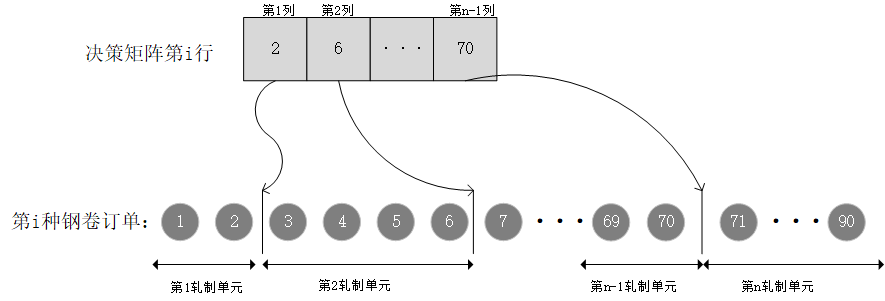
\includegraphics[width=\textwidth]{figures/bianma.png}
			\caption{插板式编码示意图}\label{lssssabel}
		\end{figure}
		
		
		\subsubsection{NSGA-II算法}
		NSGA-II算法是经典群智能多目标优化算法,其基于遗传算法与快速非支配排序,可高速有效的多目标优化的帕累托前沿。设定种群染色体数量为$p$,搜索代数为$G$,变异概率为$p_m$,$f_1(X)$、$f_2(X)$和$f_3(X)$分别为决策$X$分别表示染色体$X$所对应的转炉、连铸机于热压机的闲置产能。$T(X)$为染色体$X$对应的总流程消耗时间,其算法流程图如~\ref{111sad1sssss11}~所示。
		
		\paragraph{step1:}种群初始化
		

		首先随机生成$p$个满足所有约束条件的解作为初始化种群,即对于随机生成的第$q(1\leqslant q\leqslant p)$个染色体$X_q$有
		\begin{gather*}
	    x_{q,i,j}=floor(rand(0,N_i+1)),
		\end{gather*}
		其中$x_{q,i,j}$表示$X_q$中的第$i$行第$j$列的编码因子,$rand(0,N_i+1)$表示$0$到$N_i+1$之间的一个随机数,$floor$表示向下取整函数,即$x_{q,i,j}$为$0$到$N_i$之间的一个随机整数。将生成后个体的编码因子按行降序排列,即
		\begin{gather*}
		[x_{q,i,1},x_{q,i,2},\cdots,x_{q,i,n-1}]\leftarrow sort([x_{q,i,1},x_{q,i,2},\cdots,x_{q,i,n-1}]),
		\end{gather*}
		若所得的$X_q$满足所有约束条件,即将$X_q$保存至初始种群,生成下一个解$X_{q+1}$;否则即重复生成$X_{q}$直到其满足所有约束条件。

		
		\paragraph{step2:}交叉变异操作
		
		本文采用中间数交叉来执行隔板的交叉操作,即对个体$X_a$与个体$X_b$执行交叉操作,生成个体$X_c$,具体操作为
		\begin{gather*}
		x_{c,i,j}=x_{a,i,j}+floor((x_{b,i,j}-x_{a,i,j})\times rand(0,1)),
		\end{gather*}
		即交叉生成的基因 $x_{c,i,j}$将取自两个对应的父代基因$x_{a,i,j}$与$x_{b,i,j}$的之间的一个随机整数,将第$k$代中的所有个体两两配对进行交叉操作。之后对于第$k$代的任意一个个体$X_q$将有$p_m$的概率执行变异操作如下
		\begin{gather*}
		x_{q,i,j}(k)=floor(rand(0,N_i+1)),
		\end{gather*}
		即将$x_{q,i,j}(k)$随机变化为另一个$0$到$N_i$间的一个随机整数。将第$k$交叉变异生成的新染色体与第$k$代的原染色体混合生成染色体集合$\left \{ X \right \}_k$。
		\paragraph{step3:}快速非支配排序
		
	     若解$X_a$与$X_b$满足$\forall v\in\{1,2,3\}:f_v(X_a)\leqslant f_v(X_a)\wedge \exists v\in\{1,2,3\}:f_v(X_a)< f_v(X_a)$ ,则定义解$X_a$支配解$X_b$。若解$X_q$不被任何解支配,则称解$X_q$为非支配解。定义染色体集合$\left \{ X \right \}_k$中所有非支配解为第$1$非支配层$\left \{ X \right \}_k(1)$。剔除$\left \{ X \right \}_k$中的第$1\sim i$支配层,定义$\left \{ X \right \}_k$中剩余的解中的非支配解为第$i+1$非支配层$\left \{ X \right \}_k(i+1)$。对于第$i$支配层中的解$X_q\in \left \{ X \right \}_k(i)$,其拥挤度$C(X_q)$可计算如下
	     \begin{gather*}
	   C(X_q)=\sum_{v\in\{1,2,3\}} \frac { f_{v}(X_{q+1})- f_{v}(X_{q-1})} { f_{v,max}\left \{ X \right \}_k(i)- f_{v,min}\left \{ X \right \}_k(i)},
	     \end{gather*}
	     其中$f_{v,max}\left \{ X \right \}_k(i)$与$f_{v,min} \left \{ X \right \}_k(i)$分别是第$i$支配层中$f_{v}$的最大值与最小值。 $f_{v}(X_{q+1})$与$f_{v}(X_{q-1})$分别是第$i$支配层中解的$f_{v}$值升序排列后$f_{v}(X_{q})$的前一个与后一个值。当$f_{v}(X_{q})$即既为为$f_{v}$的最大值或最小值时使得$C(X_q)$值趋近于无穷。即将$\left \{ X \right \}_k$按照支配层编号升序排序,之后将每个支配层中的个体按照拥挤度$C(X_q)$降序排列,最终选择序列中的前$p$个个体放入下一次迭代。
	     
	     \paragraph{step4:}循环迭代寻优与选解
	     
	     循环迭代$G$次后输出第$G$代中的第$1$非支配层$\left \{ X \right \}_G(1)$,将其作为算法求得的帕累托前沿。并选择帕累托前沿解中锻造时间最小的解作为最佳生产计划。
	     \begin{figure}[H]
	     	\centering
	     	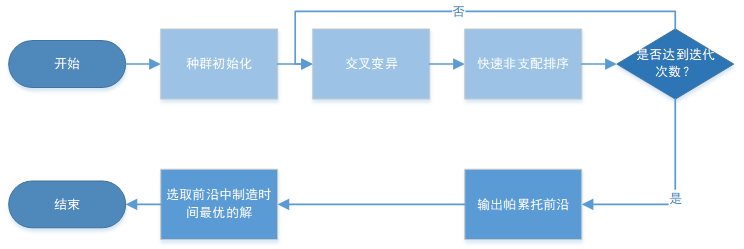
\includegraphics[width=\textwidth]{figures/liuz.png}
	     	\caption{NSGA-II算法流程图}\label{111sad1sssss11}
	     \end{figure}



\newpage
        \section{仿真实验与结果及分析}
       \subsection{实验数据及参数设置}
        本文以某钢铁联合企业为研究对象进行测试,系统使用Python编程实现算法。仿真过程中NSGA-Ⅱ算法参数设置每个种群大小为200,交叉概率为50\%, 变异概率为 80\%在CPU Intel T5800 1.6GHz, 2GB内存环境下进行多次实验,具体设置参数如表~\ref{biaozi}~所示:
        
        \begin{table}[H]
        	\setstretch{1.4}  %设置表的行间距
        	\centering		
        	\caption{实验参数设置表}\label{biaozi}
        	\begin{tabular}{cccc}
        		\toprule[2pt]
        		\multicolumn{1}{m{3cm}}{\centering 参数名称}
        		& \multicolumn{1}{m{3cm}}{\centering 参数值}
        		&  \multicolumn{1}{m{3cm}}{\centering 参数名称}
        		& \multicolumn{1}{m{3cm}}{\centering 参数值}
        		\\
        		\midrule[1pt]
        		交叉率 & 0.5 & 变异率& 0.8\\ 
        		迭代次数 &500 &种群大小 & 200\\ 
        		惩罚值 &10000 &突变领域 & 10\\ 
        		边界拥挤距离 &inf &订单数目 & 10\\ 
        		连铸设置时间 &20min &热轧设置时间 & 10min\\ 
        		轧制一块板胚时间 &2min &浇铸一块板胚时间 & 5min\\ 
        		\bottomrule[2pt]	
        	\end{tabular}
        \end{table}
        

        \subsection{实验结果}
	在充分满足各阶段生产工艺约束的条件下, 该算法能在10min内完成得到13个轧制单元计划 、 63个炉次计划和7个浇次计划,经快速非支配排叙后最终得到的Pareto非支配解有11个最优解,如图~\ref{fissssg}~所示
  	\begin{figure}[H]
  	\centering
  	\subfigure{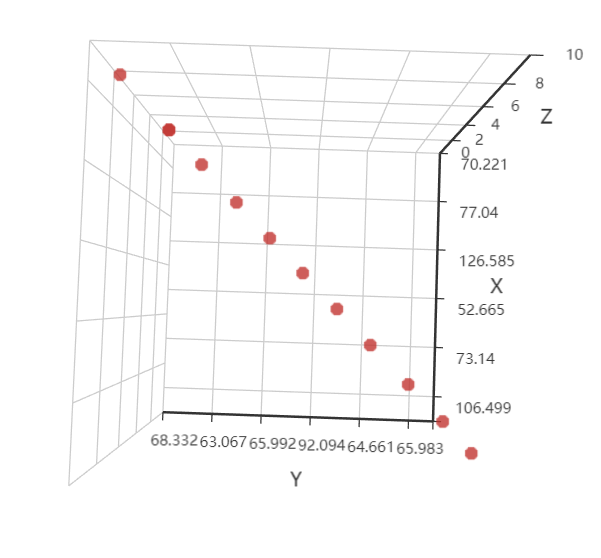
\includegraphics[height=7cm,width=7.5cm]{figures/y1.png}}
  	\subfigure{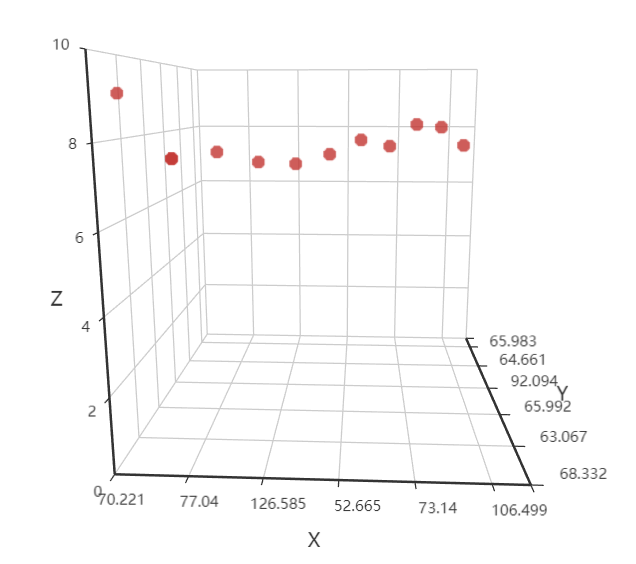
\includegraphics[height=7cm,width=7.5cm]{figures/y2.png}}
  \end{figure}	
  \begin{figure}[H]	
  	\centering
  	\subfigure{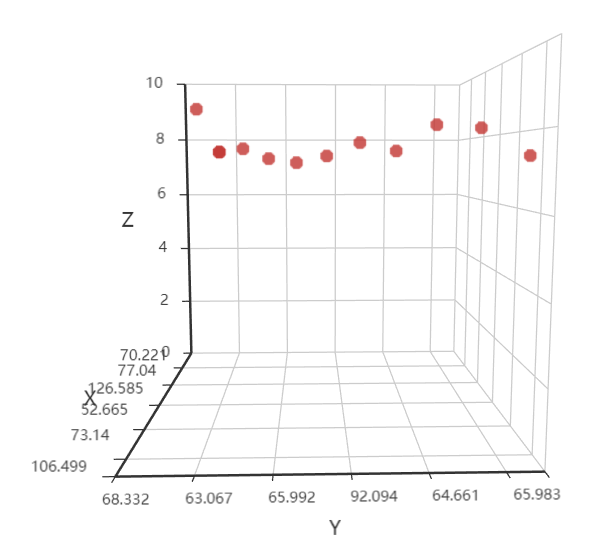
\includegraphics[height=7cm,width=7.5cm]{figures/y3.png}}
  	\subfigure{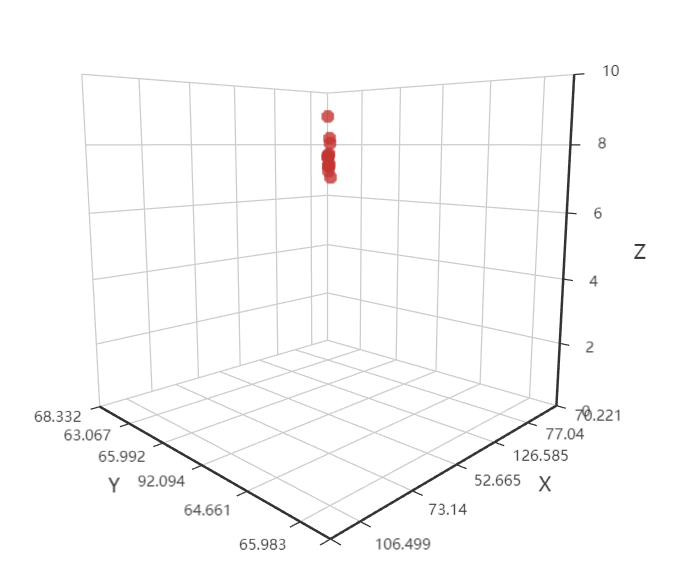
\includegraphics[height=7cm,width=7.5cm]{figures/y4.png}}
  	\caption{三维Pareto最优解散点各平面分布(缩放比例1:100)}
  	\label{fissssg}
  \end{figure}

从三维图面上可以看出,这11个Pareto解满足互不支配关系(即任意两个样本点,至少存在一轴优于另一样本点)。对于炼钢、连铸、热轧三者利用率而言,均为最优解。本文选取时间最短的一个样本点进行计算,求得满足上述约束下完成前十个订单的最短时间为36580min,其对应的插板方式如表~\ref{biasssozi}~所示

        \begin{table}[H]
	\setstretch{1}  %设置表的行间距
	\centering		
	\caption{求得最短时间热轧单元计划插板方式}\label{biasssozi}
	\begin{tabular}{c|cccccc}
		\toprule[2pt]
		\multicolumn{1}{m{4cm}}{\centering \diagbox{套餐个数}{订单号}}
		& \multicolumn{1}{m{1.5cm}}{\centering 001}
		&  \multicolumn{1}{m{1.5cm}}{\centering 002}
		& \multicolumn{1}{m{1.5cm}}{\centering 003}
		& \multicolumn{1}{m{1.5cm}}{\centering $\cdots$}
		& \multicolumn{1}{m{1.5cm}}{\centering 009}
		& \multicolumn{1}{m{1.5cm}}{\centering 010}
		\\
		\midrule[1pt]
		轧制单元1 & 43 & 11& 54&$\cdots$&12&29\\ 
		轧制单元2 &52 &30 & 109&$\cdots$&32&62\\ 
		轧制单元3 &145&88 &147&$\cdots$&47&100\\ 
		轧制单元4 &236&101 & 198&$\cdots$&61&116\\ 
		 $\cdots$&$\cdots$ &$\cdots$ & $\cdots$&$\cdots$&$\cdots$&$\cdots$\\ 
		轧制单元9&558 &167 & 508&$\cdots$&113&350\\ 
		轧制单元10 &609&188 & 593&$\cdots$&113&362\\ 
		轧制单元11 &626 &191& 648&$\cdots$&113&362\\ 
		轧制单元12 &629 &193& 656&$\cdots$&114&336\\ 
		\bottomrule[2pt]	
	\end{tabular}
\end{table}

表中纵列为插板位置所在方式,即共有12+1个轧制单元,每个轧制单元中对应订单板胚个数为横列差值求和,所得数据满足实际组炉组浇工艺约束。
	\begin{figure}[H]
	\centering
	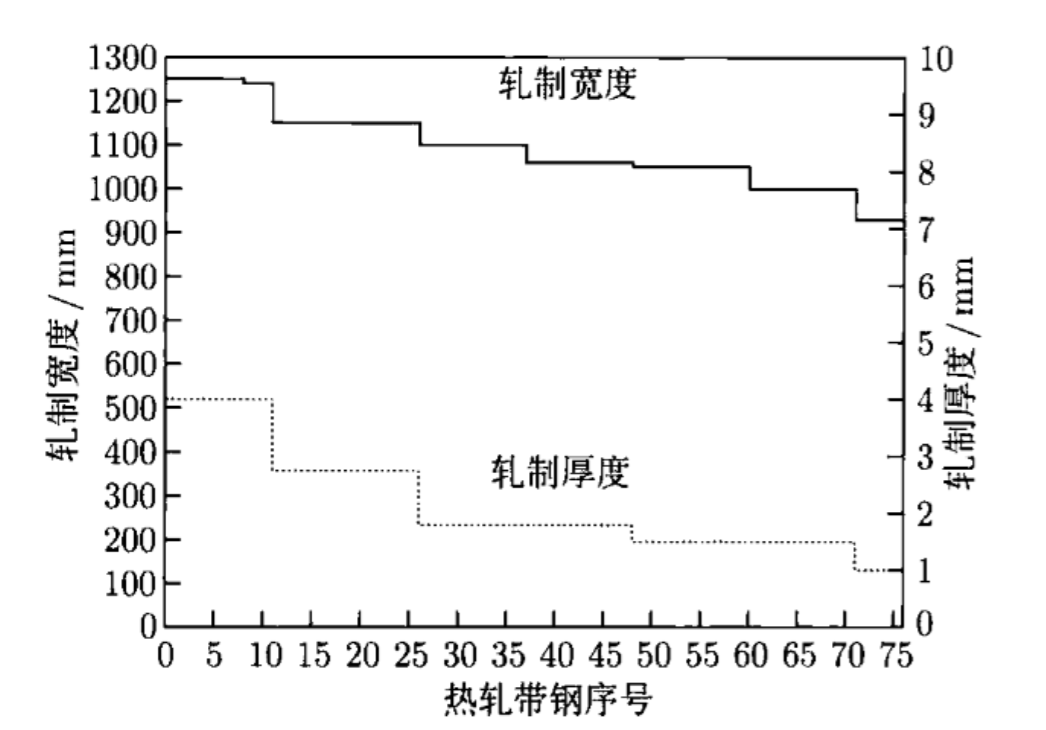
\includegraphics[width=.8\textwidth]{figures/ad.png}
	\caption{某一轧制单元宽度和厚度变化}\label{fisadsssg}
\end{figure}

 图~\ref{fisadsssg}~所表示的某轧制单元计划主体材轧制宽度和厚度的变化情况,满足轧制生产工艺约束。仿真实例计算结果检验了模型和算法的合理性、可行性和有效性。


  	\section{灵敏度分析}
 改变一体化调度系统插板个数,使其满足在约束范围内上下波动5\%。观察在固定生产订单总数的情况下,非劣解的个数和位置是否发生改变,并求出对应情况下最短生产时间。下图表示插板个数分别为11、12、13、14和15时候对应Pareto最优解分布情况。

 
 	\begin{figure}[H]
 	\centering
 	\subfigure{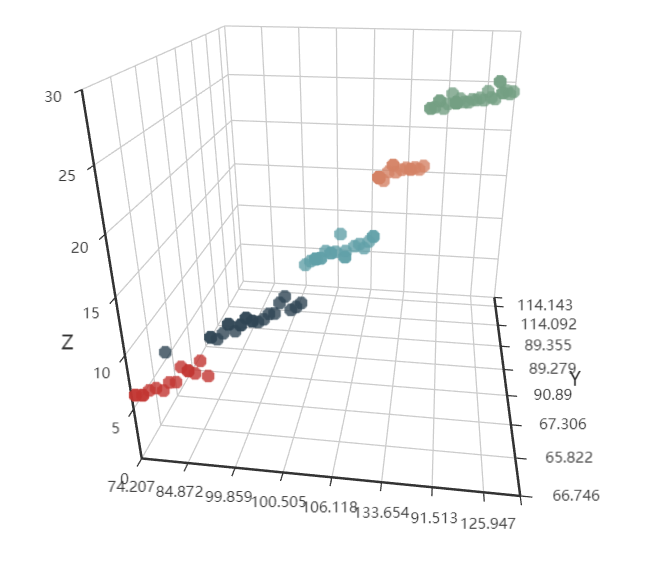
\includegraphics[height=7cm,width=7.5cm]{figures/z1.png}}
 	\subfigure{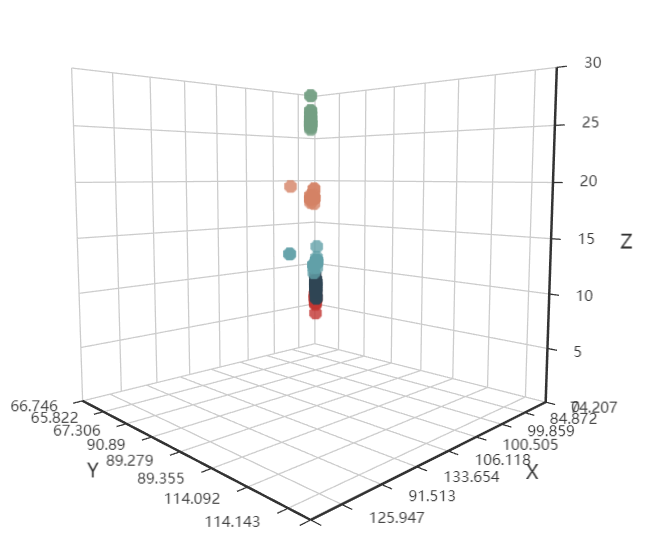
\includegraphics[height=7cm,width=7.5cm]{figures/z2.png}}
 \end{figure}	
 \begin{figure}[H]	
 	\centering
 	\subfigure{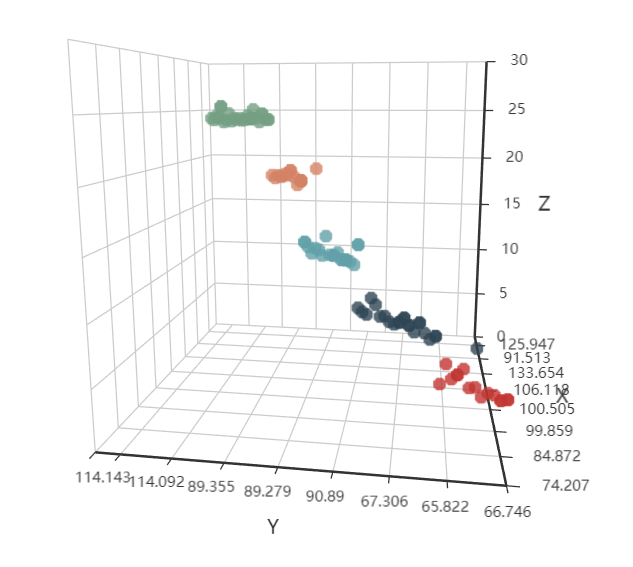
\includegraphics[height=7cm,width=7.5cm]{figures/z3.png}}
 	\subfigure{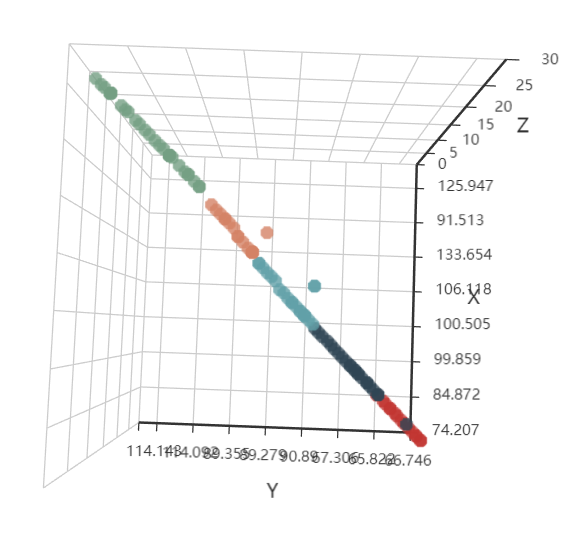
\includegraphics[height=7cm,width=7.5cm]{figures/z4.png}}
 	\caption{改变插板个数对非劣解的影响(缩放比例1:100)}
 	\label{fisadssassg}
 \end{figure}
 据图~\ref{fisadssassg}~分析可知,变化插插板个数在波动5\%时,帕累托前沿解集空间位置发生改变,但其分布并没发生较大变动,说明NSGA-II算法具有较强的抗干扰能力,在隔板参数发生改变情况下不会影响非劣解的稳定。图~\ref{xdffadaasdx}~是改变参数情况下最短生产时间的变化规律,表明在隔板参数为12情况下求得在工序间的停留最短时间,并且隔板数目对帕累托前沿解中锻造最短时间的影响较大。
 
 \begin{figure}[H]
 	\centering
 	\subfigure{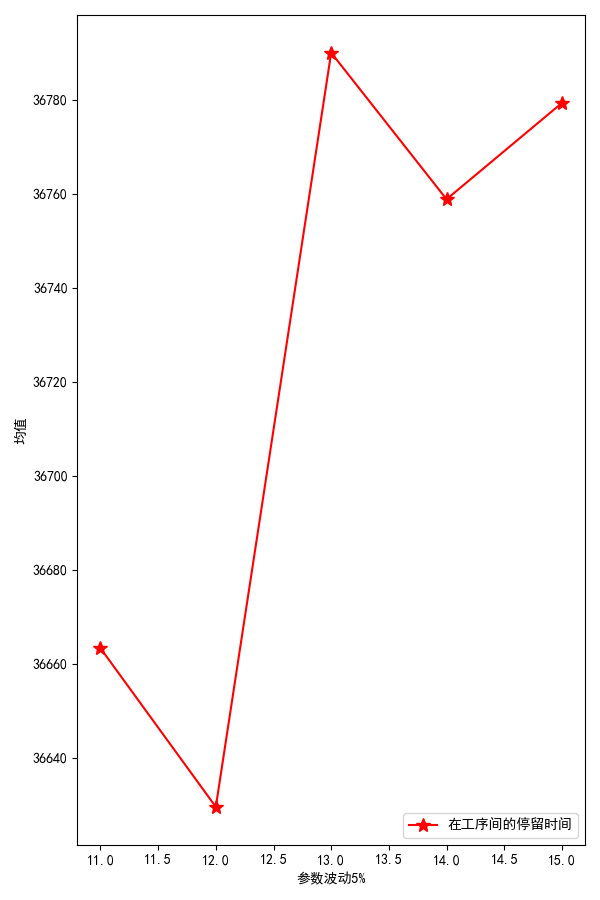
\includegraphics[width=5cm]{figures/a1.png}}
 	\subfigure{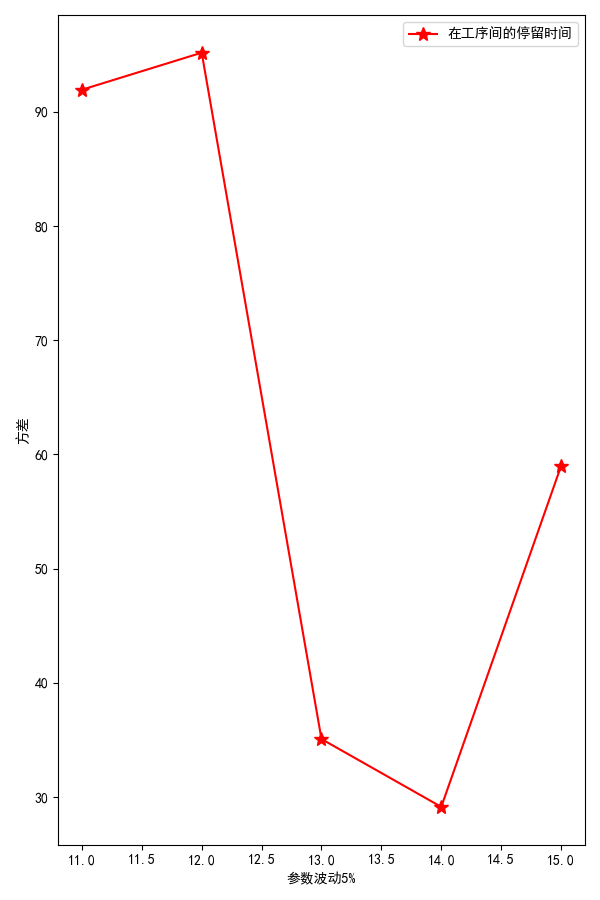
\includegraphics[width=5cm]{figures/a2.png}}
 	\subfigure{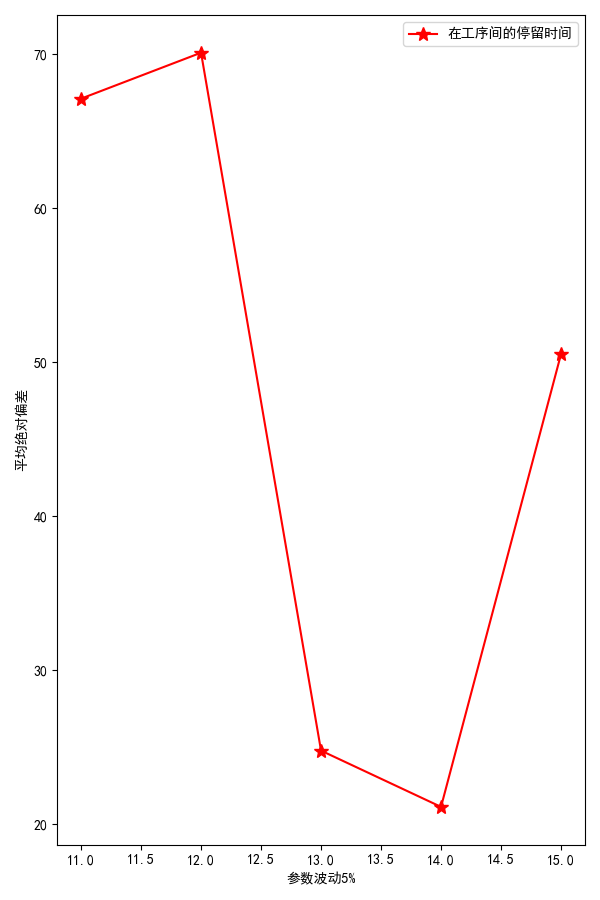
\includegraphics[width=5cm]{figures/a3.png}}
 	\caption{隔板参数变化时灵敏度分析}\label{xdffadaasdx}
 \end{figure}
 
  	\section{模型评价}
		\subsection{模型的优点}
			\begin{itemize}                                             
			\item [1.]在一体化模型的搭建中,本文多维度考虑了生产效率对全局的依赖,并在符合严苛的工艺约束条件下全局求解单元计划排列顺序。
			\item [2.] 	针对智能算法求解方面,使用NSGA-II算法并巧妙采用插板式编码方式对多目标优化求解,兼顾局部搜索与全局搜索能力。
			\item [3.] 选择帕累托前沿解中锻造时间最小的解作为最佳生产计划,求得在工序间的停留最短时间,缩短了制造周期和交货周期。
			\end{itemize}
		
		\subsection{模型的缺点}
					\begin{itemize}                                             
			\item [1.]未能考减少温降和能量损失对钢铁生产计划的影响;
			\item [2.] 	由于约束条件严苛,NSGA-II算法需要规模较大的种群数寻找满足条件的最优解,从而影响其搜索能力。
		\end{itemize}
	

 
%	\newpage	%换页符
	%%参考文献
	%\begin{thebibliography}{9}%宽度9
	% \setlength{\itemsep}{-2mm}
		\addcontentsline{toc}{section}{参考文献}
	\nocite{*}		%排版未引用的参考文献
	\begin{thebibliography}{9}%宽度9
		\bibitem{1}李文兵, 毕英杰, 纪扬, 等. 基于生产流程的炼钢-连铸-热轧仿真系统[J]. 冶金自动化, 2005, 29(3): 37-42.
		\bibitem{2}Funakawa Y, Shiozaki T, Tomita K, et al. Development of high strength hot-rolled sheet steel consisting of ferrite and nanometer-sized carbides[J]. ISIJ international, 2014, 44(11): 1945-1951.
		\bibitem{3}张春生, 李铁克. 炼钢与热轧调度方案动态协调方法研究[J]. 冶金自动化, 2016 (5): 19-25.
		\bibitem{4}朱宝琳, 于海斌. 炼钢—连铸—热轧生产调度模型及算法研究[J]. 计算机集成制造系统, 2003, 9(1): 33-36.
		\bibitem{5}李耀华, 胡国奋, 王伟, 等. 炼钢-连铸-热轧一体化生产计划编制方法研究[J]. 控制工程, 2005, 12(6): 549-552.
		\bibitem{6}李铁克, 苏志雄. 炼钢连铸生产调度问题的两阶段遗传算法[J]. 中国管理科学, 2009, 17(5): 68-74.
	\end{thebibliography}

	\newpage
	%附录
	\appendix %%附录
	\section{NSGA-II仿真实验代码}

			\lstinputlisting[language={python},numbers=left,numberstyle=\tiny,
			rulesepcolor=\color{red!20!green!20!blue!20},  
			keywordstyle=\color{blue!70!black},  
			commentstyle=\color{blue!90!},  
			basicstyle=\ttfamily] {./code/untitled0.py}

\end{document}